% !TEX root = ../Main.tex


\chapter{Introductory Material}
\label{chapterlabel1}


\begin{figure}[H]
\centering
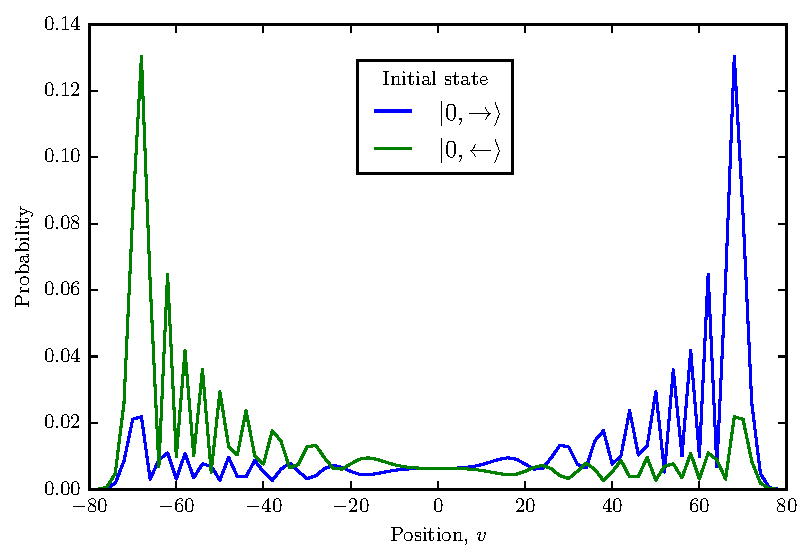
\includegraphics[width=0.8\textwidth]{hadamard_walk.pdf}
\caption{A sample figure\index{figure}.}
\end{figure}

\newcommand{\ra}[1]{\renewcommand{\arraystretch}{#1}}
\begin{landscape}
	\begin{table*}\centering
	\ra{1.3}
	\begin{tabular}{@{}rrrrcrrrcrrr@{}}\toprule
	& \multicolumn{3}{c}{$w = 8$} & \phantom{abc}& \multicolumn{3}{c}{$w = 16$} &
	\phantom{abc} & \multicolumn{3}{c}{$w = 32$}\\ \cmidrule{2-4} \cmidrule{6-8} \cmidrule{10-12}
	& $t=0$ & $t=1$ & $t=2$ && $t=0$ & $t=1$ & $t=2$ && $t=0$ & $t=1$ & $t=2$\\ \midrule
	$dir=1$\\
	$c$ & 0.0790 & 0.1692 & 0.2945 && 0.3670 & 0.7187 & 3.1815 && -1.0032 & -1.7104 & -21.7969\\
	$c$ & -0.8651& 50.0476& 5.9384&& -9.0714& 297.0923& 46.2143&& 4.3590& 34.5809& 76.9167\\
	$c$ & 124.2756& -50.9612& -14.2721&& 128.2265& -630.5455& -381.0930&& -121.0518& -137.1210& -220.2500\\ $dir=0$\\
	$c$ & 0.0357& 1.2473& 0.2119&& 0.3593& -0.2755& 2.1764&& -1.2998& -3.8202& -1.2784\\
	$c$ & -17.9048& -37.1111& 8.8591&& -30.7381& -9.5952& -3.0000&& -11.1631& -5.7108& -15.6728\\
	$c$ & 105.5518& 232.1160& -94.7351&& 100.2497& 141.2778& -259.7326&& 52.5745& 10.1098& -140.2130\\ \bottomrule
	\end{tabular}
	\caption{A sample table\index{table}}
	\end{table*}
\end{landscape}


\nocite{*}

\section{A section}
\subsection{A subsection}